\subsection{Descripción del problema.}

\vspace*{0.3cm}

Dado un \textbf{tablero de ajedrez de tamaño $n$x$n$ y $k$ caballos ocupando
inicialmente ciertos casilleros (aleatorios)} del mismo, el objetivo consiste
en \textbf{reunir a todos los caballos en un mismo casillero, minimizando la
cantidad total de movimientos realizados}. Esta cantidad equivale a
\textbf{la suma de los movimientos de todos los caballos} en el tablero.

Un caballo $k$ puede moverse únicamente \textbf{respetando los movimientos
válidos según las reglas del ajedrez}. Además, \textbf{un casillero puede
estar ocupado por más de un caballo simultáneamente}.

\vspace*{0.5cm}

\textbf{Ejemplos:}

En un tablero de 8x8, con 3 caballos en las posiciones [2,2], [5,5] y [2,8],
la menor cantidad de saltos posibles es 4, haciendo que los caballos de los
extremos cayan hacia la posición del caballo del medio, como se puede ver
en la siguiente imagen:

\begin{figure}[htb]
  \begin{center}
      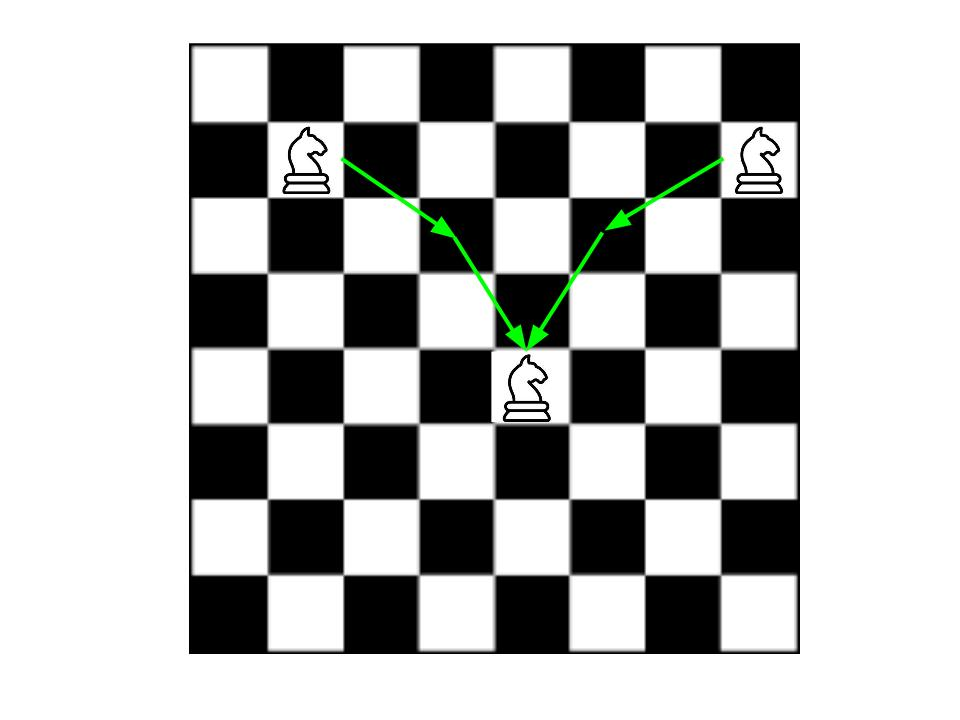
\includegraphics[scale=0.25]{imagenes/caballos.jpg}
  \end{center}
  \caption{ejemplo de tablero.}
\end{figure}


\newpage
\subsection{Desarrollo de la idea y pseudocódigo.}

\vspace*{0.3cm}


Para resolver este problema, utilizaremos $k$ tableros de $n$x$n$ casilleros,
uno por cada caballo. En cada tablero se calculará el costo para dicho caballo
de llegar a cada casillero, aplicando \textit{BFS} desde el casillero inicial,
quedando inválidos los casilleros que no pueden alcanzarse.

Luego se recorren todos los casilleros, sumando el valor de éstos en todos los
tableros (si son alcanzables), obteniendo así el costo de cada casillero para
cada caballo. De existir, el mínimo de estos valores será el casillero que
pueden alcanzar todos los caballos en la menor cantidad de saltos.

%\begin{codebox}
%\Procname{$\proc{puntoDeEncuentro}(caballos, n)$}
%\li $\id{tableros} \gets \emptyset$
%\li \For $caballo \in caballos$
%\li   \Do
%\li       $\proc{agregar}(\proc{crearTablero}(caballo,n), tableros)$
%      \End
%\li $\id{i} \gets 0$
%\li $\id{j} \gets 0$
%    $\id{min_i} \gets -1$
%    $\id{min_j} \gets -1$
%    $\id{min} \gets -1$
% \li \While $\id{i} < \id{n}$
% \li   \Do
% \li     \While $\id{j} < \id{n}$
% \li       \Do
% \li         $\id{sum} \gets 0$
% \li         $\id{caballo} \gets 0$
% \li         \While $\id{caballo} < \proc{tamaño}(caballos)$
% \li           \Do
%                 if (tableros[caballo][i][j] == -1)
%                   sum = -1
%                 else if (sum != -1)
%                   sum += tableros[caballo][i][j]
%                 end
%                 caballo++
%               \End
%             if (sum != -1 && (min == -1 || sum < min))
%               min = sum
%               min_i = i
%               min_j = j
%             end
%             j++
%         \End
%         i++
%       \End
%     if min == -1
%       \Return 'no'
%     else
% \li \Return min min_i min_j
% \end{codebox}
%
%
% crearTablero



\newpage
\subsection{Justificación de la resolución y demostración de correctitud.}

\vspace*{0.3cm}

Se dirá que el problema tiene solución cuando exista al menos un casillero del
tablero que sea alcanzable por todos los caballos, pues, siendo finitos
casilleros y sabiendo cuántos saltos le toma a cada caballo llegar a cada
casillero, se toma el mínimo de la suma de los saltos entre todos los casilleros
accesibles por todos los caballos.

Es fácil ver que el problema tiene solución para todos los tableros de tamaño
mayor a $4 \times 4$. \textcolor{red}{\textbf{Lucas, poné la demo ¿?}}.

Si, dado un caballo, se sabe la cantidad mínima de saltos que le toma llegar a
cada casillero del tablero, es sencillo obtener la solución: se recorre cada
casillero, realizando la suma ...

A continuación se probará que el algoritmo propuesto calcula, para cada caballos,
la cantidad mínima de saltos que le toma llegar a cada casillero.


\newpage
\subsection{Análisis de complejidad.}

\vspace*{0.3cm}

\textcolor{red}{\textbf{completar!}}



\newpage
\subsection{Experimentación y gráficos.}

\vspace*{0.3cm}

\subsubsection{Test 1 - benchmark caso aleatorio}

\textcolor{red}{\textbf{completar!}}


\newpage
\subsubsection{Test 2 - benchmark del peor caso}

\textcolor{red}{\textbf{completar!}}


\newpage
\subsubsection{Test 3 - benchmark del mejor caso}

\textcolor{red}{\textbf{completar!}}
